% This is LLNCS.DOC the documentation file of
% the LaTeX2e class from Springer-Verlag
% for Lecture Notes in Computer Science, version 2.4
\documentclass{book}
\usepackage{hyperref}
\usepackage{titlesec}
\usepackage[latin1]{inputenc}
\usepackage{graphicx}
\usepackage{epigraph}
\usepackage{siunitx}
\usepackage[demo]{graphicx}
\usepackage{subcaption}
\usepackage[spanish, mexico]{babel}
\usepackage{cancel}
\usepackage{amssymb}
\usepackage{booktabs}
\usepackage{amsmath}
\usepackage[thmmarks, amsmath, thref]{ntheorem}
\usepackage{color,soul}
\usepackage{animate}
\usepackage{enumitem}
\decimalpoint
\usepackage[singlelinecheck=false]{caption}
% \usepackage{multirow}
% Rename table of contents

\renewcommand{\contentsname}{Tabla de Contenidos}

% Large chapter names and number

\makeatletter
\renewcommand{\@chapapp}{Cap\'itulo}
\makeatother

% Rename part to Parte

\renewcommand{\partname}{Parte}


\newcommand{\placetitlepicture}{} % initialization

% Change references name

\renewcommand{\bibname}{Bibliograf\'ia}

% Change name of figures

\renewcommand{\figurename}{Figura}

% Declare L, M, T

\DeclareSIUnit{\length}{L}
\DeclareSIUnit{\mass}{M}
\DeclareSIUnit{\time}{T}

\DeclareSIUnit{\milla}{mi.}
\DeclareSIUnit{\inch}{in.}
\DeclareSIUnit{\pie}{ft.}
\DeclareSIUnit{\aluz}{ly.}

% Teoremas, ejercicios y ejemplos

\newtheorem{teorema}{Teorema}[section]
\theoremheaderfont{\bfseries}
\theorembodyfont{\upshape}
\theoremseparator{.}

\newtheorem{ejercicio}[teorema]{Ejercicio}
\theoremheaderfont{\bfseries}
\theorembodyfont{\upshape}
\theoremseparator{.}

\newtheorem{ejemplo}[teorema]{Ejemplo}
\theoremheaderfont{\bfseries}
\theorembodyfont{\upshape}
\theoremseparator{.}

\newtheorem*{solution*}{Soluci\'on}

%%%%%%%%%%%%%%%%%%%%%%%%%%%%%%%%%%%%%%%%%

\begin{document}

\markboth{Notas de Curso de F\'isica 1 - FF2016}{Notas de Curso de F\'isica 1 - FF2016}
\thispagestyle{empty}
% \begin{flushleft}
% \LARGE\bfseries MSc. Diego Porres\\
% Universidad del Valle de Guatemala\\[2cm]
% \end{flushleft}

\vspace{2pt}
\begin{flushright}
\Huge
\begin{tabular}{@{}l}
Notas de Curso\\
FF2016 - F\'isica 1\\
Secci\'on 130\\[6pt]
{\Large Versi\'on 0.1}
\end{tabular}
\end{flushright}
\rule{\textwidth}{1pt}
\vspace{30px}

\begin{center}
    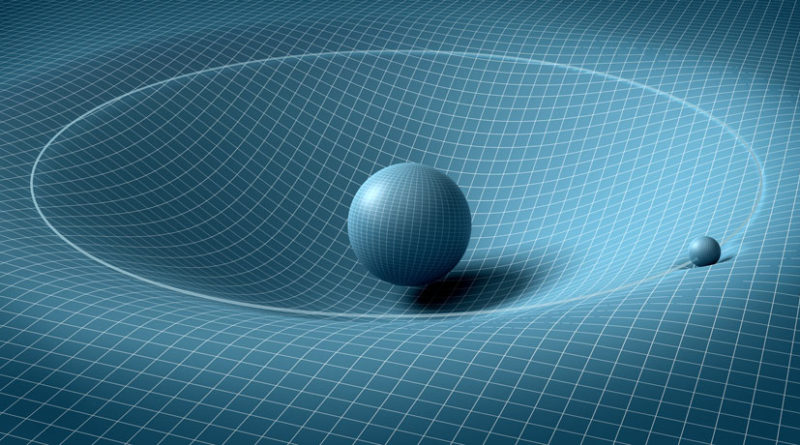
\includegraphics[width=\textwidth]{grel.jpg}
\end{center}
\vfill

\begin{flushleft}
\large\itshape
\begin{tabular}{@{}l}
{\Large\upshape\bfseries MSc. Diego Porres}\\[8pt]
Universidad del Valle de Guatemala\\[5pt]
Guatemala, Guatemala\\[5pt]
\end{tabular}
\end{flushleft}
\newpage
%
\thispagestyle{empty}
\vspace*{\fill}
\subsection*{Datos de contacto \'utiles:}
%
\begin{flushleft}
\begin{tabular}{l@{\quad}l@{\hspace{3mm}}l@{\qquad}l}
$\bullet$&\multicolumn{3}{@{}l}{\bfseries MSc. Diego Porres}\\[1mm]
&\multicolumn{3}{@{}l}{Para dudas del curso y/o errata de estas notas}\\[0.5mm]
 & e-mail:    & \href{mailto:daporres@uvg.edu.gt}{daporres@uvg.edu.gt} \\[1mm]
 & Sal\'on de clase: & A-202 \\
 & Laboratorio: & C-115 \\ [2mm]
\noalign{\rule{\textwidth}{1pt}}
\noalign{\vskip2mm}

$\bullet$&\multicolumn{3}{@{}l}{\bfseries Auxiliares de Laboratorio}\\[1mm]
&\multicolumn{3}{@{}l}{Para dudas de pr\'acticas por venir}\\[0.5mm]
 & \textbf{Mar\'ia Ren\'ee Loarca}:    & \href{mailto:marrelg22@gmail.com}{marrelg22@gmail.com} \\[1mm]
 & \textbf{Jorge Mario Tezen}: & \href{mailto:jtezen1393@gmail.com}{jtezen1393@gmail.com} \\ [2mm]

\noalign{\rule{\textwidth}{1pt}}
\noalign{\vskip2mm}
%
%{\tt svserv@vax.ntp.springer.de}\hfil first try the \verb|help|
%command.

$\bullet$&\multicolumn{3}{@{}l}{\bfseries Departamento de F\'isica:}\\[1mm]
         &\multicolumn{2}{@{}l}{Contacto: Olga Marina Castellanos}\\[0.5mm]
 & Sitio web:    & \url{http://www.uvg.edu.gt/cchh/fisica/} \\[0.5mm]
 & Tel\'efono:           & 2364-0336 Ext. 21560 \'o 21563\\[0.5mm]
 & Oficina: & C-113\\




\end{tabular}
\end{flushleft}


%
\newpage
\tableofcontents
\newpage
%
\chapter{Pr\'ologo}
% \chapter{Pr\'ologo}
%
Estas notas de curso est\'an dise\~nadas para guiar al estudiante universitario que, por primera vez, se encuentra cara a cara contra los diversos temas vistos en un curso normal de F\'isica 1. Dichos temas abarcar\'an las \'areas de mec\'anica, an\'alisis vectorial, trabajo, energ\'ia y fluidos, entre otros. 

Se espera que el estudiante tenga buen manejo del \'algebra, as\'i como de an\'alisis gr\'afico, num\'erico y geom\'etrico, pero tambi\'en se espera que el estudiante los desarrolle y se mejore al mismo tiempo a lo largo del curso.

\section{Composici\'on del Curso}

Primero lo primero: las notas. Si bien el programa del curso es bien detallado, hay algo muy sensible a dejar claro desde el inicio: \textbf{no habr\'an puntos extras, bajo ning\'un motivo}. La mayor\'ia de la nota ($57\%$) vendr\'a de los tres ex\'amenes parciales y ex\'amen final, valiendo 14 puntos cada parcial y 15 puntos el final. Habr\'an dos revisiones de sus notas de clase, i.e. de su cuaderno, por lo que se sugiere que lo tengan consigo tanto para las clases te\'oricas como para los laboratorios.

A lo largo del curso, habr\'an comprensiones de lectura, o Gu\'ias de Comprensi\'on Lectora (GCL). \'Estas se les entregar\'an

Las tareas/hojas de trabajo les ser\'an entregadas tanto en forma f\'isica como en forma digital, ya sea enviadas por correo o subidas a Canvas. Todos los documentos, incluidas estas notas de curso, ser\'an subidas y actualizadas con frecuencia a Canvas, as\'i que se le pide al alumno que revise con frecuencia \'este medio. Es posible que algunas tareas consistan en que el estudiante revise su propia tarea, siempre que se le proporcione el solucionario con anticipaci\'on. De ser as\'i, la nota consistir\'a en llenar un formulario en Google Forms (el link ser\'a proporcionado via un correo electr\'onico), as\'i como la entrega de la tarea en forma f\'isica. Se proporcionar\'a el solucionario y el estudiante, al llenar el formulario de Google Forms, reflexionar\'a si tuvo o no alg\'un problema y si tiene dudas persistentes. Se espera que el estudiante sea honesto y escriba cualquier duda que tenga, con el fin de ayudarlo a entender el tema lo antes y de la mejor manera posible.

En la semana de clases previa a cada ex\'amen parcial habr\'a un respectivo simulacro. Dicho simulacro consistir\'a en un per\'iodo de clase dedicado a resolver preguntas del mismo nivel que los parciales, y en el siguiente per\'iodo se har\'a la resoluci\'on de los mismos. La nota de los primeros dos simulacros ser\'a dividida en $50\%$ para la correcci\'on de los ejercicios, y $50\%$ para la reflexi\'on de los errores cometidos. Para el \'ultimo simulacro, la nota ser\'a $100\%$ en la reflexi\'on de los errores.

Los laboratorios ser\'an los viernes de $7:00$ a.m. a $9:25$ a.m. en el C-115. Debido a que existen 5 minutos de descanso entre per\'iodo, se juntar\'an \'estos al final para as\'i salir 10 minutos antes, es decir, a las $9:15$ a.m., para evitar cualquier confusi\'on.

Debido a pol\'iticas internas del departamento de F\'isica, los auxiliares \textbf{NO} podr\'an responder un correo que est\'e dirigido a ellos \'unicamente. Si desean una respuesta a una consulta hecha v\'ia correo electr\'onico, toda conversaci\'on deber\'a de enviarse con copia a mi correo. \'Esto es para prevenir cualquier malentendido y asegurarse que todas las partes est\'en enteradas de cualquiera que sea la duda.

\paragraph{Libro de texto: Serway \& Jewett, \textit{F\'isica para ciencias e ingenier\'ia}, 10a edici\'on, Vol. 1, 2017}

\begin{center}
    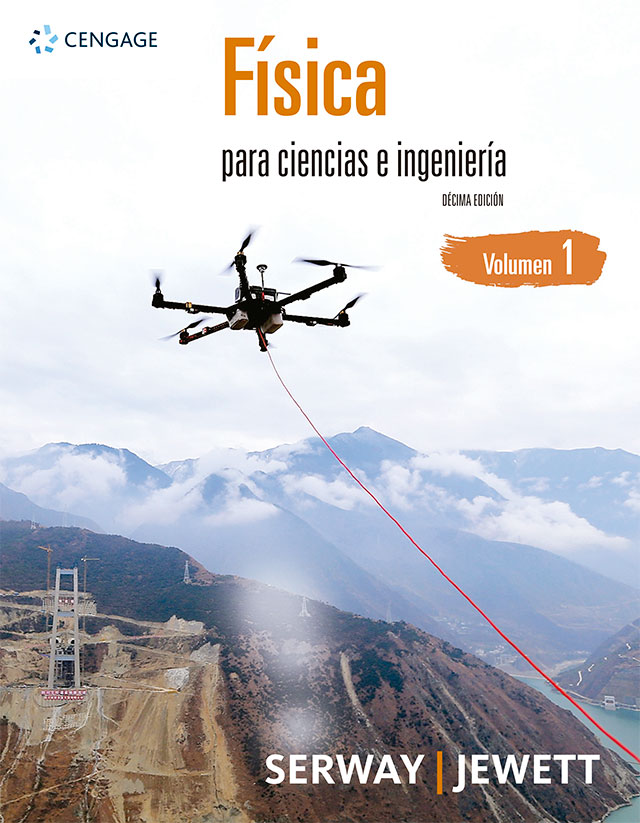
\includegraphics[width=0.65\textwidth]{serwayjewett.JPG}
\end{center}

\newpage
%
% -1	\part{part}
% 0	\chapter{chapter}
% 1	\section{section}
% 2	\subsection{subsection}
% 3	\subsubsection{subsubsection}
% 4	\paragraph{paragraph}
% 5	\subparagraph{subparagraph}

\part{Mec\'anica}\label{part:mecanica}

\chapter{F\'isica y Medici\'on}\label{ch:fisicamedicion}
%\chapter{F\'isica y Medici\'on}\label{ch:fisicamedicion}
%

\epigraph{All science is either physics or stamp collection.}{\textit{Ernest Rutherford}}

?`Qu\'e tanto sabemos realmente de nuestro Universo? ?`C\'omo podemos asegurarnos de que lo que descubramos sea cierto en otro momento en la historia, as\'i como en otras condiciones f\'isicas? ?`Es realmente necesario conocer a profundidad la historia de la tecnolog\'ia y conocimiento que tenemos hoy en d\'ia, o basta con concertrarnos en futuros experimentos? ?`Se nace uno siendo cient\'ifico, o se cultiva \'este tipo de pensamiento?

\section{Introducci\'on}\label{sec:intro1}

En el Cap\'itulo 1 de su libro de texto, se introducen un poco las \'areas en las cuales est\'a descompuesta el \'area de la F\'isica; quiz\'a podemos ahondar un poco m\'as en el tema. Si bien la F\'isica estudia todo fen\'omeno que podemos encontrar en la naturaleza, sus or\'igenes datan \'unicamente en aquellos fen\'omenos que se pod\'ian observar directamente. ?`C\'omo es posible, entonces, que podamos generar (y generalizar) ideas que sean aplicables para fen\'omenos naturales que a\'un no podamos observar o inclusive que nunca podremos observar directamente?

Si bien \'esta duda no es \'unica para la F\'isica, es una que ha persistido a lo largo de su historia. En efecto, la importancia de la F\'isica radica en su objetivo principal de estudiar los principios b\'asicos de la naturaleza y expresar a \'estos en el lenguaje de la \textit{matem\'atica}. El prop\'osito de \'esto es simple: poder predecir y por lo tanto, manipular, a la naturaleza para nuestra ventaja, adem\'as de la belleza intr\'insica que \'esto posee.

Si bien \'esto \'ultimo suena algo l\'ugubre, no lo es: teniendo \textbf{modelos} de fen\'omenos f\'isicos podremos, por ejemplo, estudiar errores pasados en la construcci\'on de puentes\footnote{Destrucci\'on del Puente de Tacoma Narrows en 1940, WA, EE.UU. \href{https://goo.gl/NyR1jp}{https://goo.gl/NyR1jp}} y as\'i evitar posibles p\'erdidas humanas (sin mencionar las materiales). Es de notar, entonces, que las caracter\'isticas que deseamos en nuestros modelos es que se utilizen la menor cantidad de conceptos, ecuaciones y suposiciones y que sean lo m\'as general posibles.

Respecto a \'este \'ultimo punto, debemos de hacer \'enfasis en lo siguiente: los modelos que generemos \textbf{\emph{NO}} son sustituto para el problema original. En efecto, s\'olo son simplificaciones de \'este para as\'i poder llegar a una soluci\'ion de una manera simple. \'Esto no quiere decir que las soluciones a las que lleguemos sean err\'oneas, sino que simplemente no ser\'an \emph{absolutamente precisas}, s\'olo hasta cierta tolerancia. Otro punto a hacer \'enfasis en la F\'isica (y Ciencias Naturales en general), es que s\'olo porque una teor\'ia tenga evidencia a su favor no quiere decir que sea infalible. Al contrario, se busca siempre encontrar posibles experimentos donde las teor\'ias fallen para as\'i descartar aquellas que no sean siempre generales. 

Cuando las predicciones hechas por los modelos son simplemente err\'oneos, entonces sabremos que las suposiciones no se est\'an cumpliendo o bien que la teor\'ia/modelo no es el adecuado. Es de recalcar, entonces, que si las suposiciones b\'asicas de nuestros modelos no se cumplen, entonces es il\'ogico esperar que los modelos se cumplan\footnote{Sobre la crisis econ\'omica del 2008: \href{https://goo.gl/jLb52T}{https://goo.gl/jLb52T}}.

Es as\'i como han nacido algunas de las distintas \'areas en las que se descompone la F\'isica. A grandes rasgos, \'estas son:

\begin{description}
    \item [Mec\'anica cl\'asica] Desarrollada principalmente por Isaac Newton (1642-1727). Es el \'area de la F\'isica que estudia el movimiento de los objetos "grandes" ($\gg\SI{e-9}{\meter}$) y que viajen a velocidades mucho menores del de la luz en el vac\'io ($\ll\SI{299792458}{\meter/\second}$). V\'ease Figura \ref{fig:mec_clasica} y Figura \ref{fig:newt_v_einst}.
    
\begin{figure}
\centering
\begin{subfigure}{.45\textwidth}
  \centering
  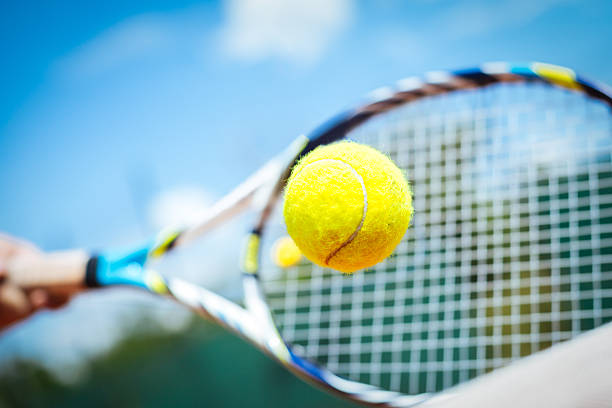
\includegraphics[width=.95\textwidth]{lecture1/tennis.jpg}
  \caption{La trayectoria de una pelota de tennis puede ser descrita sin tener que recurrir a teor\'ias avanzadas}
  \label{fig:sub_tennis}
\end{subfigure}%
\hfill
\begin{subfigure}{.45\textwidth}
  \centering
  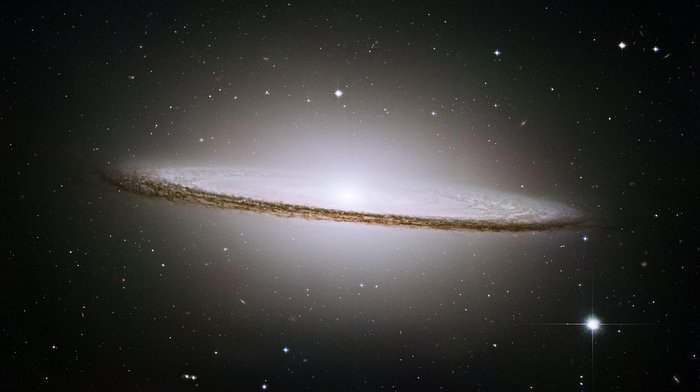
\includegraphics[width=.95\textwidth]{lecture1/sombrero.jpg}
  \caption{La Galaxia Sombrero, o Messier 104 (M104). Cr\'editos NASA/ESA y el Hubble Heritage Team}
  \label{fig:sub_galaxia}
\end{subfigure}
\caption{Dos objetos, si bien de tama\~nos abismalmente distintos, que pueden ser descritos utilizando las ecuaciones de la Mec\'anica Cl\'asica.}
\label{fig:mec_clasica}
\end{figure}
    
    \item [Relatividad] Teor\'ia generada por Albert Einstein (1879-1955) que puede describir todo objeto grande ($\gg\SI{e-9}{\meter}$) que viaje a cualquier velocidad\cite{einstein} (Mec\'anica Relativista). Sin embargo, impone un l\'imite superior a la velocidad: la de la luz ($c=\SI{299792458}{\meter/\second}$). V\'ease las Figuras \ref{fig:newt_v_einst} y  \ref{fig:aceleradores}.
    
\begin{figure}
\centering
\begin{subfigure}{.45\textwidth}
  \centering
  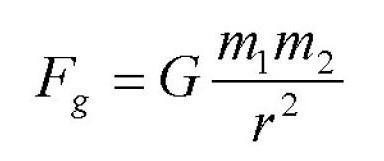
\includegraphics[width=\textwidth]{lecture1/newtongrav.jpg}
  \caption{La Ley de Gravitaci\'on Universal de Newton, la cual podremos llegar a ver m\'as adelante en este curso.}
  \label{fig:sub_newton}
\end{subfigure}%
\hfill
\begin{subfigure}{.45\textwidth}
  \centering
  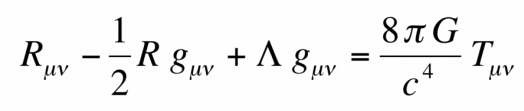
\includegraphics[width=\textwidth]{lecture1/einsteinfieldeq.jpg}
  \caption{Las Ecuaciones de Campo de Einstein.}
  \label{fig:sub_einstein}
\end{subfigure}
\caption{Dos ecuaciones que describen la interacci\'on gravitacional entre dos objetos, como se muestra en la portada de \'estas notas de curso. ?`Cu\'al escoger\'ia usted para modelar correctamente la trayectoria de un sat\'elite de GPS? ?`Por qu\'e?}
\label{fig:newt_v_einst}
\end{figure}
    
    \item [Termodin\'amica] \'Area de la F\'isica desarrollada con el fin de incrementar la eficiencia de las m\'aquinas de vapor por el franc\'es Nicolas L\'eonard Sadi Carnot (1796-1832). Las \'areas de inter\'es son el calor, el trabajo, la temperatura y el comportamiento estad\'istico de los sistemas con gran n\'umero de part\'iculas (Mec\'anica Estad\'istica).
    \item [Electromagnetismo] Teor\'ia generada por James Clerk Maxwell (1831-1879) al unir las dos \'areas que previamente se cre\'ian que eran separadas: electricidad y magnetismo. V\'ease la Figura \ref{fig:aceleradores}.
    
\begin{figure}
\centering
\begin{subfigure}{.45\textwidth}
  \centering
  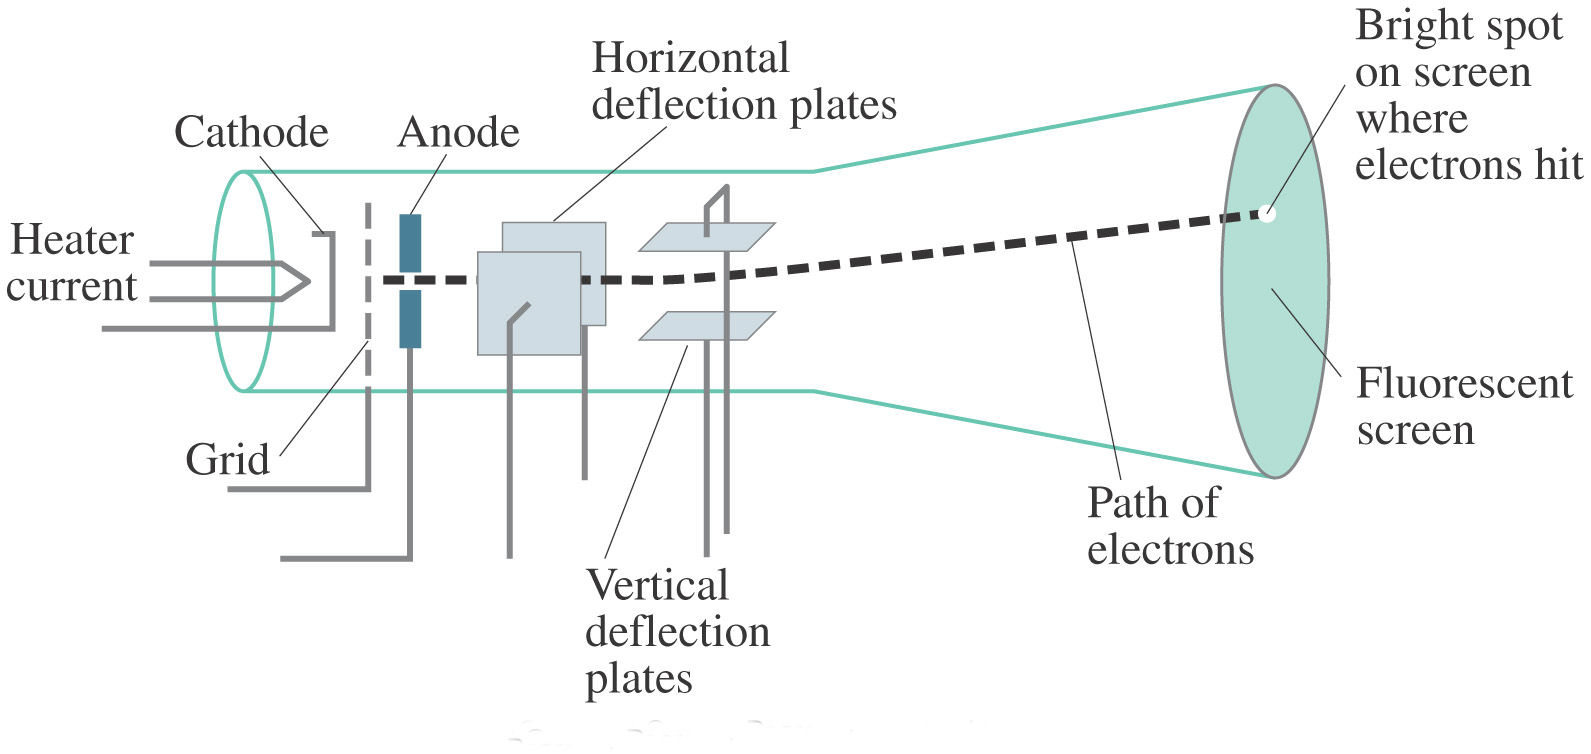
\includegraphics[width=\textwidth]{lecture1/Cathode-Ray-Tube-Diagram.jpg}
  \caption{Los primeros televisores usaban un peque\~no acelerador de part\'iculas llamado tubo de rayos cat\'odicos.}
  \label{fig:sub_cathode}
\end{subfigure}%
\hfill
\begin{subfigure}{.45\textwidth}
  \centering
  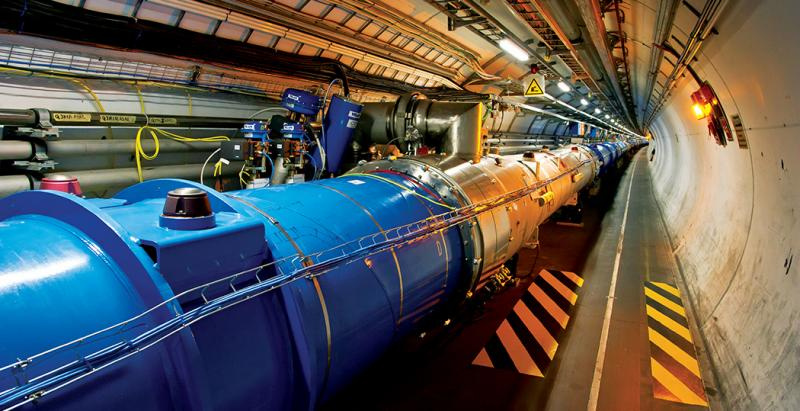
\includegraphics[width=\textwidth]{lecture1/lhc_long.jpg}
  \caption{El Gran Colisionador de Hadrones (LHC) en Ginebra, Suiza.}
  \label{fig:sub_lhc}
\end{subfigure}
\caption{Si bien la teor\'ia de Maxwell no ha cambiado, la tecnolog\'ia si lo ha hecho y se \href{https://horizon-magazine.eu/article/physicists-accelerate-plans-new-large-hadron-collider-three-times-big_en.html}{planea en seguir avanzando}.}
\label{fig:aceleradores}
\end{figure}

    \item [\'Optica] \'Area de la F\'isica que se encarga del estudio de la luz y su interacci\'on con distintos materiales.
    \item [Mec\'anica cu\'antica] Teor\'ia generada de manera separada por varios cient\'ificos a partir del siglo XVII. Es el \'area de la F\'isica que estudia el movimiento de los objetos "peque\~nos" ($\ll\SI{e-9}{\meter}$)\footnote{El por qu\'e se busca otra tecnolog\'ia para hacer transistores menores a \SI{7}{\nano\meter}, \href{https://goo.gl/WRqFmD}{https://goo.gl/WRqFmD}. } y que viajen a velocidades mucho menores del de la luz en el vac\'io  ($\ll\SI{299792458}{\meter/\second}$). Si bien existen experimentos mentales \href{http://www.fisicafundamental.net/misterios/gato.html}{famosos}, \'esta \'area tiende a ser categ\'oricamente   \href{http://cosmology.com/ConsciousTime107.html}{malinterpretada}.
\end{description}

Si bien \'esta lista no es exhaustiva, cubre la mayor\'ia de las \'areas en las cuales se descompone el \'area de la F\'isica actual. Recu\'erdese que una teor\'ia m\'as general no siempre reemplazar\'a a otra m\'as simple: en efecto, para calcular la trayectoria de un proyectil, utilizaremos las ecuaciones de la Mec\'anica Cl\'asica y no las de Einstein, ya que \'esto implicar\'ia solamente desperdiciar esfuerzos y recursos. Sin embargo, no es de sorprenderse de que se descarten algunas de estas teor\'ias en el futuro por otras teor\'ias m\'as generales.

%
\section{Est\'andares de Longitud, Masa y Tiempo}\label{sec:estandares1}
%

Debido a que queremos expresar a las teor\'ias y leyes de la F\'isica usando el lenguaje de las matem\'aticas, ciertas cantidades f\'isicas aparecen de vez en cuando. \'Estas se dividen en \emph{cantidades fundamentales} y \emph{cantidades deducidas}, donde las \'ultimas pueden ser expresadas como una combinaci\'on de las primeras. En la Mec\'anica, las tres cantidades fundamentales son \textbf{longitud}, \textbf{masa} y \textbf{tiempo}.

Si bien queremos \emph{reproducir} los resultados obtenidos previamente por nosotros o otro grupo investigativo, o viceversa, debemos de definir cierto \emph{est\'andar}. En 1960, se cre\'o el \textbf{Sistema Internacional} o \textbf{SI} (Syst\`eme International) en el cual se definieron las unidades de longitud, masa y tiempo son el \textbf{metro} (\SI{}{\meter}), el \textbf{kilogramo} (\SI{}{\kilogram}) y el \textbf{segundo} (\SI{}{\second}), respectivamente. Otros est\'andares de SI establecidos fueron las de la temperatura (el \emph{kelvin} \SI{}{\kelvin}), corriente el\'ectrica (el \emph{ampere} \SI{}{\ampere}), la intensidad luminosa (la \emph{candela} \SI{}{\candela}) y la cantidad de sustancia (el \emph{mol} \SI{}{\mole}).

Para las cantidades fundamentales de la Mec\'anica, se han acoplado los siguientes est\'andares:

\begin{description}
    \item [Longitud] En Octubre de 1983, se [re]defini\'o el metro \SI{}{\meter} como \textbf{la distancia recorrida por la luz en el vac\'io durante un tiempo de \SI{1/299792458}{\second}}.
    \item [Masa] Se estableci\'o el kilogramo \SI{}{\kilogram} en 1887 como \textbf{la masa de un cilindro de aleaci\'on platino-iridio espec\'ifico que se conserva en la Oficina Internacional de Pesos y Medidas (BIPM) en S\`evres, Francia}.
    \item [Tiempo] En 1967, se [re]defini\'o al segundo \SI{}{\second} utilizando un \emph{reloj at\'omico} de la siguiente manera: \textbf{\SI{9192631770}{} veces el per\'iodo de vibraci\'on de la radiaci\'on del \'atomo de cesio 133}.
\end{description}

Si bien \'estas definiciones parecen ser algo rebuscadas, al parecer lo son para los nuevos est\'andares internacionales. En efecto, se \href{https://www.bipm.org/utils/common/pdf/SI-statement.pdf}{redefinir\'an todas las unidades del SI en Noviembre del presente a\~no}. Se espera que \'estas redefiniciones entren en vigor el 20 de Mayo de 2019. En res\'umen, las redefiniciones del kilogramo, ampere, kelvin y mol ser\'an basadas en t\'erminos de siete constantes f\'isicas, de la misma manera en que el metro est\'a basado en la velocidad de la luz. A ra\'iz de \'esto, las unidades de SI no tendr\'an que ser modificadas conforme las mediciones e instrumentaci\'on avanzen en el futuro. 

En las Tablas \ref{table:distancias1}, \ref{table:masas1} y \ref{table:tiempos1}, se presentan algunas medidas de distintos rangos de longitud, masa e intervalos de tiempo. Tener a la mano \'este tipo de valores o tablas es importante ya que nos servir\'a para poder discernir si los resultados que obtenemos est\'an en un rango aceptable, o bien si existe la posibilidad de que se cometi\'o un error en el camino.

\begin{table}[ht]
\caption{Valores aproximados de algunas longitudes medidas}
\begin{tabular}{l r}
\toprule
           & \textbf{Longitud (\SI{}{\meter})} \\
\midrule
Di\'ametro del Universo Observable & $8.8\times10^{26}$\\
Distancia de la Tierra a la galaxia m\'as cercana (Andr\'omeda) & $2\times10^{22}$\\
Distancia del Sol a la estrella m\'as cercana (Pr\'oxima Centauri)  &  $4\times10^{16}$  \\
Radio orbital promedio de la Tierra alrededor del Sol &  $1.50\times10^{11}$ \\
Radio del agujero negro Sagitario $A^*$ en el centro de la V\'ia L\'actea & $1.2\times10^{10}$\\
Radio medio de la Tierra & $6.37\times10^{6}$\\
Altitud t\'ipica s.n.m. de un sat\'elite que orbita la Tierra & $2\times 10^5$\\
Longitud de una mosca & $5\times10^{-3}$\\
Tama\~no de las c\'elulas de la mayor\'ia de los seres vivos & $\sim10^{-5}$ \\
Di\'ametro de un \'atomo de hidr\'ogeno & $\sim10^{-10}$\\
Di\'ametro de un prot\'on & $\sim10^{-15}$\\
\bottomrule
\end{tabular}
\label{table:distancias1}
\end{table}

\begin{table}[t]
\caption{Masas aproximadas de varios objetos}
\begin{tabular}{l r}
\toprule
           & \textbf{Masa (\SI{}{\kilogram})} \\
\midrule
Universo Observable & $\sim10^{52}$\\
V\'ia L\'actea & $\sim10^{42}$\\
Gargantua (\emph{Interstellar})  &  $2\times10^{38}$  \\
Sagitario $A^*$ &  $4.31\times10^{36}$ \\
Sol & $1.99\times10^{30}$\\
Tierra & $5.98\times10^{24}$\\
Humano & $\sim 10^2$\\
Mosquito & $\sim10^{-5}$\\
Bacteria & $\sim10^{-15}$ \\
\'Atomo de hidr\'ogeno & $1.67\times10^{-27}$\\
Electr\'on & $9.11\times10^{-31}$\\
\bottomrule
\end{tabular}
\label{table:masas1}
\end{table}


\begin{table}[t]
\caption{Valores aproximados de algunos intervalos de tiempo}
\begin{tabular}{l r}
\toprule
           & \textbf{Intervalo de Tiempo (\SI{}{\second})} \\
\midrule
Edad del Universo & $4.35\times10^{17}$\\
Edad de la Tierra & $1.43\times10^{17}$\\
Un a\~no  &  $3.2\times10^{7}$  \\
Un d\'ia (revoluci\'on de la Tierra sobre su eje) &  $8.6\times10^{4}$ \\
Un per\'iodo de clase & $2.7\times10^{3}$\\
Latido normal & $8\times10^{-1}$\\
Tiempo que le toma a un prot\'on dar una vuelta al LHC & $\sim 10^{-4}$\\
Intervalo de tiempo para que la luz cruze un prot\'on & $\sim10^{-24}$\\
\bottomrule
\end{tabular}
\label{table:tiempos1}
\end{table}

Adem\'as de \'estos valores normales, existen prefijos para denotar las potencias en la notaci\'on cient\'ifica y evitar potencias muy grandes o muy peque\~nas, como lo son nano (\si{\nano}), micro (\si{\micro}), centi (\si{\centi}), kilo (\si{\kilo}), mega (\si{\mega}), giga (\si{\giga}), entre otros. \'Estos no se les quedar\'an memoriz\'andose \'esta tabla, sino con la pr\'actica, as\'i como su uso diario. Para una mejor referencia, vea la Tabla 1.4 de su libro de texto.


\section{An\'alisis Dimensional}\label{sec:analisisdim1}

En la F\'isica, llamamos a la \emph{dimensi\'on} a la naturaleza f\'isica de una cantidad. Es decir, no importa si expresamos las medidas de un objeto en metros, pies o pulgadas, siempre seguimos hablando de una distancia. Lo mismo sucede para las otras dos cantidades fundamentales de masa y tiempo. 

Se utilizar\'an, entonces, a los s\'imbolos \si{\length}, \si{\mass} y \si{\time} para denotar a las dimensiones de longitud, masa y tiempo, respectivamente. Adem\'as, utilizaremos los corchetes $[\cdot]$ para denotar que estamos analizando las dimensiones de una cantidad f\'isica. Apliquemos \'esto a un ejemplo:

\begin{ejemplo}
Encuentre las dimensiones del \'area de un cuadrado de lado $a$.
\label{ej:area}
\end{ejemplo}

\begin{solution*}Aplicamos nuestro operador $[\cdot]$ a la f\'ormula o ecuaci\'on del \'area $A$ de un cuadrado:

\[ [A] = [a^2] = [a]\cdot[a] = \si{\length}\cdot\si{\length} = \si{\length}^{2} \]\hfill$\square$

\end{solution*}

Por lo tanto, el \textbf{an\'alisis dimensional} puede ser utilizado para verificar que una ecuaci\'on est\'e escrita de manera correcta, especialmente cuando veamos t\'erminos en nuestras ecuaciones que tengan potencias distintas a uno. Asimismo, nos ser\'a \'util para verificar que nuestro resultado final sea correcto, si es que existe alguna duda al respecto.

En res\'umen, el poder del an\'alisis dimensional yace en que las \textbf{dimensiones pueden ser tratadas como cantidades algebraicas}, como hemos hecho en el Ejemplo \ref{ej:area}. Dicho de otra manera, podemos sumar o restar cantidades \'unicamente si tienen las mismas dimensiones y una ecuaci\'on tiene sentido solamente si ambos lados de \'esta tienen las mismas dimensiones. 

\begin{table}[t]
\caption{Unidades y unidades de distintas cantidades deducidas}
\begin{tabular}{l ccccc}
\toprule
Cantidad  & \textbf{Vol\'umen ($V$)} & \textbf{Rapidez ($v$)} & \textbf{Aceleraci\'on ($a$)} & \textbf{Fuerza ($F$)}\\
\midrule
Dimensiones & $\si{\length}^{3}$ & $\si{\length}/\si{\time}$ & $\si{\length}/\si{\time}^{2}$ & $\si{\mass}\cdot\si{\length}/\si{\time}^{2}$\\
Unidades SI & $\si{\meter}^{3}$ & $\si{\meter}/\si{\second}$ & $\si{\meter}/\si{\second}^{2}$ & $\si{\kilogram}\cdot\si{\meter}/\si{\second}^{2}$\\
\bottomrule
\end{tabular}
\label{table:dimensiones}
\end{table}

Utilizando la Tabla \ref{table:dimensiones}, proseguimos a resolver ejemplos m\'as complejos:

\begin{ejemplo}
\textcolor{red}{\textbf{\hl{W}}} En la Figura \ref{fig:sub_newton} vemos la Ley de Gravitaci\'on de Newton, la cual nos permite calcular la fuerza gravitatoria que ejercen dos cuerpos entre s\'i, i.e.:

\[ F_{g} = G \frac{m_{1}m_{2}}{r^{2}}\]

donde $F_{g}$ es la fuerza gravitatoria, $G$ es la constante de gravitaci\'on universal de Newton, $m_{1}$ y $m_{2}$ son las masas de los dos objetos y $r$ es la distancia entre \'estos. Encuentre las dimensiones de $G$.
\label{ej:newton}
\end{ejemplo}

\begin{solution*}Aplicamos nuestro operador $[\cdot]$ a ambos lados de la ecuaci\'on y utilizando la Tabla \ref{table:dimensiones}:

\begin{align*}
    [F_{g}] &= [G \frac{m_{1}m_{2}}{r^{2}}] \\
    \implies \si{\mass}\frac{\si{\length}}{\si{\time}^{2}} &= [G] \frac{\si{\mass}^{2}}{\si{\length}^{2}}\\
    \implies [G] &= \cancel{\si{\mass}}\frac{\si{\length}}{\si{\time}^{2}} \frac{\si{\length}^{2}}{\cancel{\si{\mass}^{2}}}\\
    \therefore [G] &= \frac{\si{\length}^{3}}{\si{\mass\time^{2}}}
\end{align*} \hfill$\square$

%\si[per-mode = fraction]{\cancel\kilogram\metre\per\cancel\kilogram\per\second}

\end{solution*}

Es de notar que el an\'alisis dimensional \textbf{\emph{NO}} nos dar\'a los valores num\'ericos de las constantes en las ecuaciones, solamente sus dimensiones. Dichos valores de las constantes aparecen \'unicamente a trav\'es de la experimentaci\'on, algo que veremos en los laboratorios m\'as adelante.

\begin{ejercicio}
Una cantidad deducida es la \textbf{densidad} de un objeto de masa $m$ que ocupa un vol\'umen $V$. \'Esta se denota por $\rho$ y se calcula de la siguiente manera:

\begin{equation}
    \rho = m/V
\end{equation}

Encuentre las dimensiones en el SI para la densidad $\rho$.
\end{ejercicio}

\begin{ejercicio}
Nos dicen que la aceleraci\'on $a$ de una part\'icula de massa $m$ que se mueve a una rapidez constante $v$ en una trayectoria circular de radio $r$ es proporcional a alguna potencia de $r$ (digamos $r^{\alpha}$), a alguna potencia de $v$ (digamos $v^{\beta}$) y a alguna potencia de $m$ (digamos $m^{\gamma}$). Encuentre los valores de las potencias.
\end{ejercicio}

\section{Conversi\'on de Unidades}\label{sec:conversion1}

No todos los pa\'ises o instituciones alrededor del mundo utilizan las mismas unidades, a veces debemos de cambiar de un sistema (como el SI) a otro (como el de Unidades de medida de Estados Unidos, \href{https://es.wikipedia.org/wiki/Unidades_tradicionales_de_Estados_Unidos}{USCS}). A menos que querramos aparecer en vergonzosas listas\footnote{V\'ease, por ejemplo: \url{https://goo.gl/z35nY7}}, por no mencionar los riesgos a la vida humana. Por lo tanto, es de vital importancia que puedan realizar la conversi\'on de unidades de manera correcta. Hist\'oricamente, donde m\'as se ha visto \'esto es en su curso de Qu\'imica, por lo que espero que \'esta no sea la primera vez que vean \'este tipo de conversiones.

La conversi\'on de unidades puede ser tanto entre sistemas (SI a USCS, e.g., de kil\'ometros a millas), o bien dentro de un sistema (e.g., de metros a kil\'ometros). Algunos ejemplos de \'este tipo de conversiones entre sistemas son (pero no dude de revisar el Ap\'endice A de su libro de texto para la lista completa):

\begin{equation*}
\begin{aligned}[c]
\SI{1}{\milla}&=\SI{1609}{\meter} = \SI{1.609}{\kilo\meter}\\
\SI{1}{\meter}&=\SI{39.37}{\inch} = \SI{3.281}{\pie}
\end{aligned}
\hspace{10mm}
\begin{aligned}[c]
\SI{1}{\pie}&=\SI{0.3048}{\meter} = \SI{30.48}{\centi\meter}\\
\SI{1}{\inch} &= \SI{0.0254}{\meter} = \SI{2.54}{\centi\meter} 
\end{aligned}
\end{equation*}

Siguiendo la misma l\'inea del an\'alisis dimensional visto en la Secci\'on \ref{sec:analisisdim1}, las unidades entonces tambi\'en pueden ser tratadas como cantidades algebraicas. Es decir, podemos sumarlas siempre que sumemos metros con metros, por ejemplo, y podemos cancelarlas si se dividen entre s\'i y se trate de la misma unidad.

\begin{ejemplo}
Por alguna raz\'on, usted decidi\'o comprarle un veh\'iculo a una su conocida. Sin embargo, el indicador de velocidad muestra \'unicamente la rapidez en millas por hora (\si{\milla/\hour}). Si el l\'imite de velocidad en la carretera donde est\'a manejando es de \SI{70}{\kilo\meter/\hour} y el indicador dice que usted viaja a \SI{60}{\milla/\hour}, ?`rebas\'o usted el l\'imite de velocidad?
\end{ejemplo}

\begin{solution*}
Usando ya sea el Ap\'endice A o la peque\~na lista que les proporcion\'e anteriormente, podemos convertir las millas a kil\'ometros para as\'i convertir la rapidez en kil\'ometros por hora. Multiplicamos, entonces a la rapidez dada por un neutro multiplicativo, i.e.:

\[ \SI{60}{\milla/\hour} = 60 \frac{\cancel{\si{\milla}}}{\si{\hour}} \left(\frac{\SI{1.609}{\kilo\meter}}{1\cancel{\si{\milla}}}\right) = \SI{96.54}{\kilo\meter/\hour} \]

Es decir, EMETRA le dar\'a una jugosa multa (asumiendo que una c\'amara o polic\'ia lo haya capturado en el acto).\hfill $\square$
\end{solution*}

\begin{ejercicio}
La estrella m\'as cercana al Sol, Pr\'oxima Centauri, se encuentra a aproximadamente \SI{4e13}{\kilo\meter} de distancia. Se define a un a\~no luz (\si{\aluz}) como la distancia que recorre la luz en un a\~no. Convierta \'esta distancia de \si{\kilo\meter} a \si{\aluz}
\end{ejercicio}


\section{Estimaciones y C\'alculos de Orden de Magnitud}\label{sec:ordenmagn1}

En \href{https://www.quora.com/If-you-were-at-a-Google-interview-how-would-you-answer-How-many-views-does-YouTube-have-per-day}{las afamadas entrevistas de Google}\footnote{\'Este tipo de problemas se conocen como Problemas de Fermi en homenaje al famoso f\'isico Enrico Fermi (1901-1954).}, se han pedido a los entrevistados que estimen los valores de ciertas cantidades que parecen imposibles de calcular sin la informaci\'on necesaria. La importancia de \'estos problemas radica no en obtener c\'alculos precisos, sino en poder reconocer correctamente las hip\'otesis utilizadas previo a la realizaci\'on de los experimentos.

Dichas estimaciones se suelen expresar como una \textbf{\'orden de magnitud}, es decir, una potencia de 10. En general, para calcular el \'orden de magnitud de un n\'umero $N$, proseguimos con:

\begin{itemize}
    \item Expresar a $N$ como $N=a\times10^{b}$, con $\sqrt{10}/10\leq a < \sqrt{10}$.
    \item $b$ ser\'a la \'orden de magnitud que deseamos encontrar, con $b\in\mathbb{Z}$.
\end{itemize}

N\'otese que el resultado que obtengamos ser\'a confiable hasta dentro de un factor de 10. Utilizamos a $\sim$ para denotar que un n\'umero es "del \'orden de". Otra notaci\'on equivalente es utilizando la Notaci\'on O Grande, $\mathcal{O}$, si es que la han visto. 

\begin{ejercicio}
Verifique, entonces, que lo siguiente est\'a correcto:

\begin{equation*}
    \SI{0.0086}{} \sim 10^{-2}\equiv \mathcal{O}\left(10^{-2}\right) \hspace{5mm} \SI{0.0021}{} \sim 10^{-3} \equiv \mathcal{O}\left(10^{-3}\right) \hspace{5mm} \SI{720}{} \sim 10^{3} \equiv \mathcal{O}\left(10^{3}\right)
\end{equation*}

\end{ejercicio}

N\'otese que en las estimaciones que usted haga, las imprecisiones hechas por subestimar alg\'un n\'umero com\'unmente se contrarrestan con las sobreestimaciones hechas de otro n\'umero. S\'olo la pr\'actica permitir\'a que dichas imprecisiones sean cada vez menores, por lo que lo mejor, como con cualquier otra \'area, es practicar y practicar. Veamos, entonces, el siguiente famoso ejemplo:

\begin{ejemplo}
Estime el n\'umero de afinadores de piano en la Ciudad Capital de Guatemala.
\end{ejemplo}

\begin{solution*}
La poblaci\'on de la Ciudad Capital es aproximadamente de 3 millones de habitantes. Supongamos que, en promedio, hay 3 personas por casa, que cada 30 casas hay un piano, que cada piano es afinado una vez al a\~no, y que cada afinador realiza unas 250 afinaciones cada a\~no. Por lo tanto, en la Ciudad Capital hay:

\[
    3\times10^{6}\cancel{\text{personas}} \left( \frac{1\,\cancel{\text{casa}}}{3\,\cancel{\text{personas}}} \right) \left( \frac{1\,\cancel{\text{piano}}}{30\,\cancel{\text{casas}}} \right) \left( \frac{1\,\cancel{\text{afinaci\'on/a\~no}}}{1\,\cancel{\text{piano}}} \right) \left( \frac{1\,\text{afinador}}{250\,\cancel{\text{afinaciones/a\~no}}} \right)
\]

lo cual nos da que hay, aproximadamente, 133 afinadores en la Ciudad Capital, o bien, $\sim 10^2$ afinadores de piano. \hfill $\square$

\end{solution*}

\begin{ejercicio}
Estime el n\'umero de respiraciones tomadas por una persona durante una vida humana promedio.
\end{ejercicio}

\begin{ejercicio}
Estudie la Paradoja de Fermi e indique si est\'a de acuerdo o no con el resultado, y por qu\'e. Para referencia, puede utilizar el \href{https://waitbutwhy.com/2014/05/fermi-paradox.html}{siguiente enlace}.
\end{ejercicio}

\section{Cifras Significativas}\label{sec:cifras1}

Los valores medidos de las cantidades medidas se conocen \'unicamente dentro de los l\'imites de incertidumbre experimental. El n\'umero de \textbf{cifras significativas} nos puede indicar acerca de esta incertidumbre. En efecto, la calidad de experimentaci\'on, de los aparatos que se usaron para realizar las mediciones, e incluso la experiencia del experimentador afectan dicha incertidumbre.

Al combinar dos mediciones distintas, no tiene sentido utilizar todas las cifras de una al mismo tiempo que llenar de ceros a la otra. Por ejemplo, si hacemos la siguiente suma:

\[ \pi + 5.3 \]

la respuesta no es un n\'umero irracional con infinitas cifras (al menos no en el sentido de este curso). Por lo tanto, tendremos dos reglas generales a seguir para utilizar la cantidad correcta de cifras significativas:

\begin{itemize}
    \item \textbf{Cuando se multiplican o dividan varias cantidades, el n\'umero de cifras significativas en la respuesta final es el mismo que el n\'umero de cifras significativas en la cantidad que tiene el n\'umero m\'as peque\~no de cifras significativas.}
    \item \textbf{Cuando se sumen o resten cantidades, el n\'umero de lugares decimales en el resultado debe de ser igual al n\'umero m\'as peque\~no de lugares decimales de cualquier t\'ermino en la suma o diferencia.}
\end{itemize}

\begin{ejemplo}
Calcule el \'area de un c\'irculo de radio $r=\SI{6.0}{\centi\meter}$.
\end{ejemplo}

\begin{solution*}
Ya que el radio tiene dos cifras significativas, el resultado final debe de tener \'unicamente dos cifras significativas. Por lo tanto:
\[ A = \pi (\SI{6.0}{\centi\meter})^2 = 1.1\times10^2\si{\centi\meter}^2\]
\hfill $\square$
\end{solution*}

Los ceros pueden o no ser cifras significativas, todo depender\'a de qu\'e lado del punto decimal se encuentren. Es decir, los n\'umeros $0.0003$ y $0.0045$ tendr\'an una y dos cifras significativas, respectivamente, mientras que los n\'umeros $1.5\times10^3$ y $1.500\times10^3$ tendr\'an 2 y 4 cifras significativas, respectivamente. 

\begin{ejemplo}
Calcule las siguientes sumas o restas:

\[ 123+5.35 \hspace{15mm} 1.002-0.998 \hspace{15mm} 23.2 + 5.174\]

\end{ejemplo}

\begin{solution*}
Usando la segunda regla, tendremos los siguientes resultados:

\[ 
123+5.35 = 128 \text{, ya que el primero no tiene lugares decimales}\]
\[
1.002-0.998 = 0.004 \text{, ya que tienen el mismo n\'umero de lugares decimales}\]
\[
23.2+5.174 = 28.4 \text{, ya que el primero tiene un lugar decimal}
\]
\hfill $\square$
\end{solution*}

En el \'ultimo ejemplo, vemos que tuvimos que redondear nuestro resultado final. La regla general para redondear dice que, si el \'ultimo d\'igito eliminado es mayor que 5, aumentamos por 1 al d\'igito retenido. Si el \'ultimo d\'igito eliminado es menor que 5, entonces el \'ultimo d\'igito retenido se queda como est\'a. Por \'ultimo, si el \'ultimo d\'igito eliminado es igual a 5, el d\'igito restante debe redondearse al n\'umero par m\'as cercano.

Por \'ultimo, el consejo a tener en \'este tipo de c\'alculos es a redondear \'unicamente hasta el final, ya que redondear al introducir cada n\'umero solo aumentar\'a los errores exponencialmente. Asimismo, en su libro de texto se utilizar\'an 3 cifras significativas, para tenerlo en cuenta a la hora de entregar tareas ya sea de forma f\'isica como por WebAssign.

\begin{ejercicio}
Estime el vol\'umen del Volc\'an de Agua. D\'e su respuesta en $\si{\kilo\meter}^{3}$ y utilize 3 cifras significativas.
\end{ejercicio}


%
\chapter{Movimiento en una Dimensi\'on}\label{ch:Movimiento1d}
%\chapter{Movimiento en una Dimensi\'on}\label{ch:Movimiento1d}
%

\epigraph{...It seemed that this poor ignorant Monarch-as he called himself-was persuaded that the Straight Line which he called his Kingdom, and in which he passed his existence, constituted the whole of the world, and indeed the whole of Space. Not being able either to move or to see, save in his Straight Line, he had no conception of anything out of it...}{Edwin A. Abbott, \emph{Flatland: a Romance of Many Dimensions}}

A diferencia del personaje principal de la novela de Edwin A. Abbott, nosotros habitamos un universo con tres dimensiones espaciales (mas uno temporal). Sin embargo, muchas veces lo m\'as sencillo es empezar nuestro estudio de los fen\'omenos f\'isicos con el menor n\'umero de dimensiones, para as\'i luego ir agregando m\'as complejidad y generalidad a nuestros modelos.

Empezaremos, entonces, con el estudio de la \textbf{cinem\'atica}, el cual es una porci\'on de la Mec\'anica Cl\'asica que describe el movimiento de distintos objetos f\'isicos. Asumiremos, entonces, que la mayor\'ia de los objetos que estudiemos (si no es que todos) son \textbf{part\'iculas} o se comportan como \'estas. Es decir, que son objetos que tienen masa pero de tama\~no infinitesimal. Por ejemplo, podemos tratar a la Tierra como una part\'icula y modelar su movimiento alrededor del sol ya que el radio de la Tierra es mucho menor comparado al radio de la \'orbita que \'esta toma alrededor del Sol.

\section{Posici\'on, Velocidad y Rapidez}\label{sec:posvelrap2}

De la misma manera que tenemos un sistema de referencia para definir los est\'andares de medici\'on para comparar la longitud, masa y tiempo, tendremos un sistema de coordenadas que nos permita indicar la \textbf{posici\'on} de una part\'icula. Por lo tanto, decir que una part\'icula se encuentra a $\SI{5}{\meter}$ de distancia tiene sentido \'unicamente si decimos \emph{respecto a qu\'e}; en este caso, respecto a nosotros mismos.

T\'ipicamente denotamos con $O$ al \textbf{or\'igen} de \'este sistema de coordenadas. Por lo tanto, en el ejemplo anterior, nosotros ser\'iamos el or\'igen de nuestro eje de coordenadas. Estaremos utilizando las \emph{coordenadas cartesianas}, pero existen muchas otras m\'as (depender\'a de la simetr\'ia del problema que quieran atacar). De manera un poco arbitraria, en \'este sistema de coordenadas posicionamos a los n\'umeros positivos hacia la derecha del or\'igen, al 0 en el or\'igen, y a los negativos a la izquierda de \'este. V\'ease la Figura \ref{fig:cart2}.

\begin{figure}[ht]
\centering
  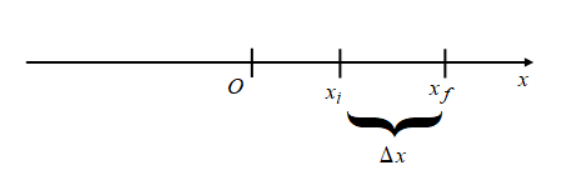
\includegraphics[width=0.8\textwidth]{lecture2/ejex.png}
\caption{Eje de coordenadas cartesianas en una dimensi\'on. Llamamos a la diferencia entre la posici\'on inicial $x_{i}$ y la final $x_{f}$ ell desplazamiento $\Delta x$. N\'otese que \'este puede ser positivo o negativo.}
\label{fig:cart2}
\end{figure}

Si tenemos, a lo largo de ciertos intervalos de tiempo, las mediciones de la posici\'on de un objeto, podemos calcular el desplazamiento de \'este. El \textbf{desplazamiento} de una part\'icula se define como su cambio en la posici\'on en un intervalo de tiempo. Es decir, que si nuestra part\'icula empieza en una posici\'on inicial $x_{i}$ y se mueve a una posici\'on final $x_{f}$, su desplazamiento estar\'a dado por:

\begin{equation}\label{eq:desplazamiento}
    \Delta x = x_{f} - x_{i}
\end{equation}

donde denotamos al desplazamiento por $\Delta x$. En general, utilizaremos a la letra griega $\Delta$ para denotar un cambio, ya sea en la posici\'on, tiempo, o cualquier otra cantidad f\'isica. N\'otese, entonces, que el desplazamiento puede ser positivo o negativo, todo depender\'a de las posiciones iniciales y finales de nuestra part\'icula (v\'ease la Figura \ref{fig:cart2}).

Es de notar el desplazamiento no es igual a la distancia recorrida por el veh\'iculo. En efecto, la \textbf{distancia} es la longitud total del camino tomado por cualquier part\'icula en un intervalo de tiempo definido (v\'ease la Figura \ref{fig:despl2}). Por lo tanto, la distancia \'unicamente puede ser cero o positiva, nunca negativa. Por lo tanto, llamamos a la distancia una \textbf{cantidad escalar} ya que solo tiene \emph{magnitud}, mientras que el desplazamiento es una \textbf{cantidad vectorial}, ya que tiene tanto \emph{magnitud} como \emph{direcci\'on}. \'Esta distinci\'on se har\'a m\'as notoria en el siguiente cap\'itulo.

\begin{figure}[ht]
\centering
  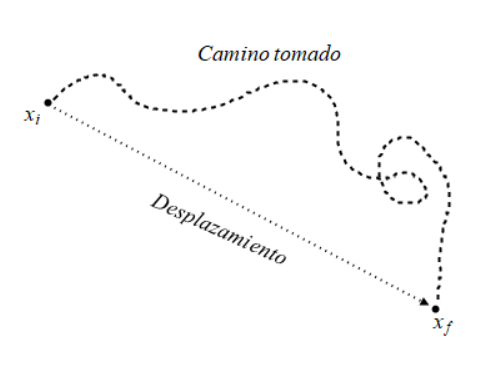
\includegraphics[width=0.8\textwidth]{lecture2/desplazamiento.PNG}
\caption{Desplazamiento entre dos puntos inicial y final, $x_{i}$ y $x_{f}$. N\'otese que la longitud del camino tomado ser\'a la distancia total recorrida $d$.}
\label{fig:despl2}
\end{figure}

Usualmente denotamos a la distancia por la letra $d$ y la escribimos de la siguiente manera (si no se siente c\'omodo a\'un con la notaci\'on, ignore la siguiente ecuaci\'on):

\begin{equation}\label{eq:distancia}
    d = \sum_{i=0}^{N}\lvert x(t_{i+1}) - x(t_{i}) \rvert = \sum_{i=1}^{N}\lvert \Delta x_{i} \rvert 
\end{equation}

Como un ejemplo sencillo para poder distinguir a la distancia y al desplazamiento, piense en su recorrido en un d\'ia normal: usted sale de su casa, hace su recorrido (se cual sea \'este) y al final, regresa a su casa. Su desplazamiento, entonces, al empezar y finalizar el d\'ia fue de cero, mas su distancia recorrida fue mayor a cero. 

\begin{ejemplo}\label{ej:carro2}
Analizemos el movimiento de un autom\'ovil que se mueve sobre el eje $x$. Las mediciones de su posici\'on las tendremos cada \SI{10}{\second}. Por lo tanto, tendremos la siguiente tabla de mediciones:

\begin{table}[ht]
\caption{Posici\'on del autom\'ovil en varios tiempos}
\begin{tabular}{l rrrr}
\toprule
\textbf{Posici\'on}  & \textbf{$t$ ($\si{\second}$)} & \textbf{$x$ ($\si{\meter}$)} & \textbf{$\Delta x$ ($\si{\meter}$)} & \textbf{$d$ ($\si{\meter}$)}\\
\midrule
$A$ & 0 & 30 & \-- & 0\\
$B$ & 10 & 52 & 22 & 22\\
$C$ & 20 & 38 & -14 & 36\\
$D$ & 30 & 0 & -38 & 74\\
$E$ & 40 & -37 & -37 & 111\\
$F$ & 50 & -53 & -16 & 127\\
\bottomrule
\end{tabular}
\label{table:carro1d2}
\end{table}

N\'otese que con s\'olo las primeras dos columnas podemos llenar las \'ultimas dos columnas de desplazamiento y distancia. Presentar la informaci\'on en forma de tabla es importante, pero el ser humano es muy visual, as\'i que proseguiremos a presentar la posici\'on del veh\'iculo en funci\'on del tiempo. V\'ease la Figura \ref{fig:posdist2}. A \'este tipo de gr\'aficas se les llama \emph{gr\'afica posici\'on-tiempo}.

\begin{figure}[ht]
    \centering
    \animategraphics[controls={play, step,stop},loop,width=0.8\textwidth]{1}{./gif/posdist/posdist-}{0}{3}
    \caption{Gr\'aficas de posici\'on del veh\'iculo y de la distancia recorrida. ?`Cu\'al es cu\'al? N\'otese que podemos generar mejores curvas que unan a los puntos, pero no necesariamente quiere decir que la posici\'on y la distancia se comporten de \'esta manera. Juegue con \'este usando Adobe Acrobat Reader.}
    \label{fig:posdist2}
\end{figure}

Es posible dibujar una curva que una todos nuestros puntos, pero a menos que sepamos exactamente c\'omo se mueve el veh\'iuclo, s\'olo ser\'ia un modelo de infinitos posibles. Por lo tanto, a\'un no podemos graficar con exactitud c\'omo se mueve el veh\'iculo, a menos que incrementemos nuestra frecuencia de muestreo (es decir, reduzcamos el intervalo de tiempo en el cual tomamos los datos).

\hfill $\square$
\end{ejemplo}

Otra forma de analizar los datos que tenemos es combinando las cantidades medidas de otra manera. N\'otese en la Tabla \ref{table:carro1d2} que en algunos tramos de la trayectoria, el veh\'iculo recorri\'o una mayor distancia que en otros.  La forma m\'as com\'un para comparar \'este tipo de movimiento es dividiendo el desplazamiento hecho, $\Delta x$, por el intervalo de tiempo durante el que ocure \'este desplazamiento, $\Delta t$. A \'esto se le llama \textbf{velocidad promedio} y se denota por $v_{x, \text{prom}}$, es decir:

\begin{equation}\label{eq:velprom2}
    v_{x, \text{prom}}\equiv \frac{\Delta x}{\Delta t}
\end{equation}

Debido a que el $\Delta t > 0$\footnote{Y a\'un no sabemos por qu\'e: \url{https://goo.gl/TtPYjZ}}, el signo de la velocidad promedio depender\'a entonces del signo del desplazamiento realizado. Por lo tanto, si la part\'icula se desplaza hacia la derecha, tendremos que $\Delta x >0$; si se desplaza hacia la izquierda, entonces $\Delta x < 0$ y si se queda quieto, entonces $\Delta x = 0$. Respectivamente, esto querr\'a decir que la velocidad promedio de la part\'icula ser\'a positiva ($v_{x, \text{prom}} > 0$), negativa ($v_{x, \text{prom}} < 0$) o igual a cero ($v_{x, \text{prom}} = 0$). N\'otese, entonces que esto implica que la velocidad ser\'a una \emph{cantidad vectorial}.

Las dimensiones de la velocidad promedio ser\'an $\si{\length/\time}$, o en el SI, $\si{\meter/\second}$. Podemos interpretar, en nuestra gr\'afica de la Figura \ref{fig:cart2}, a la velocidad promedio como la \textbf{pendiente de la l\'inea que une a dos puntos en nuestra trayectoria en nuestra gr\'afica posici\'on-tiempo}. 

Como \'ultima parte de \'esta secci\'on, definiremos un nuevo t\'ermino: la rapidez. En el d\'ia a d\'ia, es usual confundir los t\'erminos de velocidad con rapidez, pero en la F\'isica hay una gran distinci\'on. La \textbf{rapidez promedio} (una \emph{cantidad escalar}) se define como la distancia total viajada $d$ dividida por el tiempo total que se tom\'o en viajar dicha distancia, es decir:

\begin{equation}\label{eq:rapprom2}
    v_{\text{prom}}\equiv \frac{d}{\Delta t}
\end{equation}

Sus dimensiones tambi\'en ser\'an \si{\length/\time} y en el SI, \si{\meter/\second}. N\'otese, entonces, que como tratamos con una cantidad escalar, la rapidez promedio no tendr\'a signo, es decir, no tendr\'a direcci\'on: $v_{\text{prom}} \geq 0$. 

\begin{ejemplo}
Encuentre la velocidad y rapidez promedio del veh\'iculo del Ejemplo \ref{ej:carro2} entre los puntos $A$ y $F$.
\end{ejemplo}

\begin{solution*}

Nuestros puntos inicial y final ser\'an los puntos $A$ y $F$, por lo que:

\begin{equation*}
    \Delta x = x_{f}-x_{i}=x_{F} - x_{A} = \SI{-53}{\meter} - \SI{30}{\meter}=\SI{-83}{\meter}
\end{equation*}

El intervalo de tiempo durante este tramo del recorrido es:

\begin{equation*}
    \Delta t = t_{f}-t_{i}=t_{F} - t_{A} = \SI{50}{\second} - \SI{0}{\second}=\SI{50}{\second}
\end{equation*}

Por lo tanto, la velocidad promedio, usando la Ecuaci\'on \ref{eq:velprom2}, ser\'a:

\begin{equation*}
    v_{x, \text{prom}}= \frac{\Delta x}{\Delta t} = \frac{\SI{-83}{\meter}}{\SI{50}{\second}}=+\SI{1.7}{\meter/\second}
\end{equation*}

Para obtener la rapidez promedio, necesitaremos usar todos los otros puntos para calcular la distancia total recorrida por el veh\'iculo. De suerte, ya hemos calculado \'esto, por lo que $d=\SI{127}{\meter}$. Por lo tanto, la rapidez promedio ser\'a:

\begin{equation*}
    v_{\text{prom}}= \frac{d}{\Delta t} = \frac{\SI{127}{\meter}}{\SI{50}{\second}}=+\SI{2.5}{\meter/\second}
\end{equation*}

\hfill $\square$
\end{solution*}

\section{Velocidad y Rapidez Instant\'aneas}\label{sec:valrapinst2}

La velocidad y rapidez promedio no siempre son la mejor manera de analizar el movimiento de la part\'icula en cuesti\'on. En efecto, a veces deseamos conocer la rapidez o velocidad de una part\'icula \emph{en un instante}. Para \'este fin, Newton \href{https://www.youtube.com/watch?v=X_xR5Kes4Rs}{invent\'o} el C\'alculo, una poderosa herramienta que al d\'ia de hoy seguimos utilizando, inclusive para \href{https://towardsdatascience.com/gradient-descent-in-a-nutshell-eaf8c18212f0}{entrenar agentes de Inteligencia Artificial}. 

Previamente, discutimos acerca de la interpretaci\'on gr\'afica de la velocidad promedio, siendo \'esta la pendiente de la recta que une a dos puntos en la gr\'afica posici\'on-tiempo. Dicha recta se llama la \emph{l\'inea secante}. ?`Qu\'e pasar\'ia con el valor de \'esta pendiente si ambos puntos tienden a ser el mismo? V\'ease la Figura \ref{fig:secantder2}, donde tratamos de responder \'esta pregunta de manera gr\'afica.

\begin{figure}[ht]
    \centering
    \animategraphics[controls={play, step,stop},loop,width=\textwidth]{10}{./gif/tangent/tangent-}{0}{21}
    \caption{Las l\'ineas secantes y tangentes a una curva en unos puntos espec\'ificos. N\'otese que, al hacer que la distancia entre los dos puntos (rojo y azul) tiendan a cero, las pendientes de ambas l\'ineas tienden al mismo valor. Juegue con \'este usando Adobe Acrobat Reader.}
    \label{fig:secantder2}
\end{figure}

Por lo tanto, \textbf{la pendiente de la recta tangente a un punto en la curva de posici\'on de una part\'icula ser\'a su \emph{velocidad instant\'anea} en dicho punto}. Dicho de otra manera, empleando el lenguaje del C\'alculo, la velocidad instant\'anea, $v_{x}$ ser\'a la proporci\'on $\Delta x/\Delta t$ cuando $\Delta t$ tiende a cero, i.e.:

\begin{equation}\label{eq:deriv2}
    v_{x}\equiv \lim_{\Delta t\to0} \frac{\Delta x}{\Delta t}=\frac{dx(t)}{dt}
\end{equation}

La \'ultima igualdad es la notaci\'on de Leibniz y es la que m\'as utilizaremos. N\'otese que, ya que seguimos tratando con una pendiente a una curva, \'esta puede ser positiva, negativa o igual a cero, por lo que la velocidad instant\'anea seguir\'a siendo una cantidad vectorial. La \textbf{rapidez instant\'anea} ser\'a la magnitud de la velocidad instant\'anea, por lo que ser\'a una cantidad escalar. En la Tabla \ref{table:vel2} presentamos ciertos rangos de rapidez instant\'anea para saber los distintos rangos que podremos encontrar en el Universo.

\begin{table}[ht]
\caption{Rapidez de varios objetos observados}
\begin{tabular}{l r}
\toprule
           & \textbf{Rapidez (\si{\kilo\meter/\hour})} \\
\midrule
OMG Particle & $c-5.4\times10^{-15}$\\
Protones en LHC (7 TeV) & $1.079\times10^{9}$\\
S2 (orb. Sagitario $A^*$) &  $1.8\times10^{7}$ \\
PSR B2224+65 (pos. dejando la VL)  &  $5.8\times10^{6}$  \\
V\'ia L\'actea (rel. Fondo de Microondas) & $1.99\times10^6$\\
Andr\'omeda (acerc\'andose a nosotros) & $1.08\times10^6$\\
Sistema Solar alrededor de la V\'ia L\'actea & $7\times10^5$\\
Tierra alrededor del Sol & $1.07\times10^5$\\
Voyager 1 & $6.1\times10^4$\\
Rapidez de escape de la Tierra & $4.03\times10^4$\\
Estaci\'on Espacial Internacional & $2.77\times10^4$\\
Transbordador Espacial (STS) & $5.04\times10^3$\\
La Tierra (Punto en el Ecuador) & $1.67\times10^3$\\
Sonido en atm\'osfera est\'andar & $1.2\times10^3$\\
Airbus A380 & $9\times10^2$\\
Viento de un tornado grande & $468$\\
Formula Rossa (monta\~na rusa) & $240$\\
Usain Bolt (\SI{100}{\meter} en 2009) & $44.72$\\
Marcha promedio para un humano & $3.6\to5.4$\\
Crecimiento de bamb\'u & $5.0\times10^{-5}$\\
Ritmo promedio que se aleja la Luna  de la Tierra & $4.7\times10^{-9}$ \\
Deriva continental & $1\times10^{-9}\to1\times10^{-8}$\\
Ritmo de expansi\'on entre 2 puntos en el espacio a \SI{1}{\meter} & $7.8\times10^{-18}$\\
\bottomrule
\end{tabular}
\label{table:vel2}
\end{table}

De aqu\'i en adelante, utilizaremos a la palabra \emph{velocidad} para denotar a la velocidad instant\'anea y, de hablarse de la velocidad promedio, utilizaremos tal adjetivo.

\begin{ejemplo}
Una part\'icula se mueve a lo largo del eje $x$. Su posici\'on var\'ia con el tiempo de acuerdo a la expresi\'on $x=-4t+2t^2$\footnote{Lo correcto es escribir $x(t)=(-4.0\si{\meter/\second})t+(2.00\si{\meter/\second^2})t^{2.00}$, pero no est\'a mal ignorar las dimensiones de las constantes, siempre que tengan sentido desde un principio.}, donde $x$ est\'a en metros y $t$ en segundos. $a)$ Dibuje la gr\'afica posici\'on-tiempo de la part\'icula. $b)$ Calcule el desplazamiento de la part\'icula en los intervalos de tiempo de $t=0\si{\second}$ a $t=1\si{\second}$ y de $t=1\si{\second}$ a $t=3\si{\second}$. $c)$ Calcule la velocidad promedio durante estos dos intervalos de tiempo. $d)$ Encuentre la velocidad instant\'anea de la part\'icula en $t=2.5\si{\second}$.
\end{ejemplo}

\begin{solution*}
\begin{enumerate}[label=\alph*)]
    \item N\'otese que podemos escribir a la curva de la trayectoria como: $x=2t(t-2)$, por lo que la part\'icula cruzar\'a el eje $t$ cuando $t=0\si{\second}$ y  $t=2\si{\second}$. Como la curva es una par\'abola abierta hacia arriba, y por simetr\'ia, sabremos que el m\'inimo de la misma se encontrar\'a en el punto medio entre las intersecciones en el eje $t$, es decir: $x(1)=-4(1)+2(1)^2=-2\si{\meter}$. Con \'esto, podemos recrear la curva de la par\'abola:

\begin{figure}[ht]
\centering
  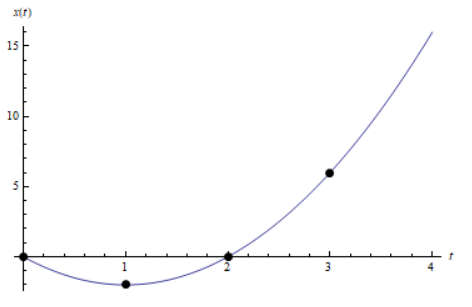
\includegraphics[width=\textwidth]{lecture2/plotparab.PNG}
\caption{Posici\'on de la part\'icula que estamos analizando en el ejercicio.}
\label{fig:plotparab2}
\end{figure}    

    \item Llamemos al punto $A$ al punto cuando $t=\SI{0}{\second}$; al punto $B$ al punto cuando $t=\SI{1}{\second}$; al punto $C$ al punto cuando $t=\SI{3}{\second}$. Entonces, tendremos que los desplazamientos son:
    
    \[ \Delta x_{A\to B} = x_{B} - x_{A} = (-4(1)+2(1)^2) - (-4(0)+2(0)^2) = -4+2=-2\si{\meter} \]
    y
    \[ \Delta x_{B\to C} = x_{C} - x_{B} = (-4(3)+2(3)^2) - (-4(1)+2(1)^2) = -12+18+4-2=+8\si{\meter} \]
    
    \item Tendremos que:
    
    \[ v_{x, \text{prom}}^{A\to B} = \frac{\Delta x_{A\to B}}{\Delta t_{A\to B}} = \frac{\SI{-2}{\meter}}{\SI{1}{\second}}=\SI{-2}{\meter/\second} \]
    y
    \[ v_{x, \text{prom}}^{B\to C} = \frac{\Delta x_{B\to C}}{\Delta t_{B\to C}} = \frac{\SI{8}{\meter}}{\SI{2}{\second}}=+\SI{4}{\meter/\second} \]
    
    \item Su libro de texto les dice, crudamente, que hay que medir la pendiente de la tangente en el punto dado. Si bien es factible, en este caso en espec\'ifico tienen a mano la curva exacta que toma la part\'icula. Por lo tanto, utilizaremos la Ecuaci\'on \ref{eq:deriv2}:
    
    \begin{equation*}
    \begin{split}
        v_{x}(t) &= \lim_{\Delta t\to0} \frac{\Delta x}{\Delta t} = \lim_{\Delta t\to0} \frac{x(t+\Delta t) - x(t)}{\Delta t}\\
        &=\lim_{\Delta t\to0}\frac{\left(-4(t+\Delta t)+2(t+\Delta t)^2\right) - \left(-4t+2t^2\right)}{\Delta t}\\
        &=\lim_{\Delta t\to0}\frac{\cancel{-4t}-4\Delta t\cancel{+2t^2}+4t\Delta t+2\Delta t^2\cancel{+4t}\cancel{-2t^2}}{\Delta t}\\
        &=\lim_{\Delta t\to0}\frac{-4\cancel{\Delta t}+4t\cancel{\Delta t}+2\Delta t^{\cancel{2}}}{\cancel{\Delta t}}\\
        &=\lim_{\Delta t\to0} \left( -4+4t+2\Delta t \right)\\
        &=-4+4t
    \end{split}
    \end{equation*}
    
    Por lo tanto, la velocidad instant\'anea en $t=\SI{2}{\second}$ ser\'a:
    
    \[ v_{x}(2.5\si{\second}) =  -4+4(2.5)=-4+10=+\SI{6}{\meter/\second}\]
    
    Pruebe medir la pendiente de la tangente de su libro de texto y comprobar que, en efecto, la pendiente es positiva y tiene valor 6.

\end{enumerate}

\hfill $\square$
\end{solution*}

\section{Modelo de An\'alisis: La part\'icula bajo velocidad constante}\label{sec:velcte2}

Cuando analizamos un carro, persona, estrella, o cualquier objeto, y reconocemos que se mueve con una velocidad constante, entonces las propiedades intr\'insicas de cada objeto no nos importan, ni nos afectar\'an en nuestros c\'alculos. \'Esto nos permitir\'a utilizar el modelo correcto, con el cual tendremos la lista adecuada de ecuaciones a utilizar \textbf{y NO viceversa}. Muchos cometen el error durante un examen, por ejemplo, de ver el listado de ecuaciones disponibles y utilizar alguna al azar. No s\'olo tendr\'an respuestas err\'oneas, sino que lo m\'as probable es que se compliquen m\'as de lo necesario.

Por lo tanto, reitero: el modelo de una \textbf{part\'icula que se mueve con velocidad constante} se puede aplicar a cualquier objeto que se puede modelar como una part\'icula que se mueve a velocidad constante, sin importar otros factores (tiene manos, es masivo, est\'a vivo, etc.).

Ya que la velocidad de la part\'icula es constante, su velocidad instant\'anea en cualquier instante durante un intervalo de tiempo ser\'a igual a la velocidad promedio durante dicho intervalo. Es decir, $v_{x}=v_{x,\text{prom}}$. 

\begin{equation*}
    v_{x}=\frac{\Delta x}{\Delta t}
\end{equation*}

Por lo tanto, usando la Ecuaci\'on \ref{eq:velprom2} y notando que en la pr\'actica utilizaremos a $t_{i}=\SI{0}{\second}$, llegamos a lo siguiente:

\begin{equation}\label{eq:velconst2}
    x_{f}=x_{i}+v_{x}t
\end{equation}

N\'otese que \'esta ecuaci\'on es la ecuaci\'on de una l\'inea recta con pendiente $v_{x}$ e intersecci\'on con el eje $x$ se da en $x_{i}$. Si se tiene la informaci\'on de que la part\'icula que se est\'a analizando se mueve a una velocidad constante, podemos r\'apidamente graficar su posici\'on como una l\'inea recta con las especificaciones previamente descritas.

\begin{ejercicio}
Una kinesi\'ologa estudia a un corredor que corre a lo largo de una l\'inea recta a un ritmo constante. Despu\'es de haber recorrido $4\si{\second}$, ella mide que el corredor se encuentra a $20\si{\meter}$ de cuando activ\'o el cron\'ometro. $a)$ ?`Cu\'al es la velocidad del corredor? $b)$ ?`Cu\'al es la posici\'on del corredor despu\'es de haber transcurrido $10\si{\second}$?
\end{ejercicio}

Una part\'icula que se mueve a \textbf{rapidez constante} no es lo mismo que una que se mueve a velocidad constante. En efecto, pueden haber casos en donde \'estos sean iguales, pero no siempre lo ser\'a debido a la naturaleza distinta de que una cantidad sea escalar y la otra vectorial. 

Continuando con la ecuaci\'on de la rapidez promedio, Ecuaci\'on \ref{eq:rapprom2}, denotaremos a la rapidez constante con $v$, por lo que:

\begin{equation}\label{eq:rapconst2}
    v = \frac{d}{\Delta t}
\end{equation}

\begin{ejemplo}
Imagine un \'aguila que circula los cielos tratando de localizar a su presa. Si se mueve a una rapidez constante de $\SI{5.00}{\meter/\second}$ y su trayectoria es circular con un radio de $\SI{10.0}{\meter}$, calcule entonces el intervalo de tiempo requerido para que el \'aguila complete un viaje alrededor del c\'irculo.
\end{ejemplo}

\begin{solution*}
Podemos utilizar la ecuaci\'on de rapidez constante, ya que sabemos que el \'aguila se mueve a rapidez constante. N\'otese que la distancia total recorrida es el per\'imetro de un c\'irculo. Por lo tanto, despejando a $\Delta t$ de la Ecuaci\'on \ref{eq:rapconst2}, tenemos que:

\[ \Delta t = \frac{d}{v} = \frac{2\pi r}{v} = \frac{2\pi(\SI{10.0}{\meter})}{\SI{5.00}{\meter/\second}} = \SI{4\pi}{\second}=\SI{12.6}{\second} \]

\hfill $\square$
\end{solution*}

\begin{ejercicio}
Calcule la rapidez promedio de la Tierra mientras \'esta gira alrededor del Sol. Utilize la Tabla \ref{table:distancias1} y note que la Tierra recorre \'esta distancia en 1 a\~no. ?`Cu\'anta distancia recorre la Tierra, entonces, en un d\'ia?
\end{ejercicio}

\section{Propuesta de modelo de an\'alisis para resolver problemas}

Su libro de texto propone unos pasos (modelo de an\'alisis) para poder llegar a la resoluci\'on de un problema a la hora de enfrentarse a \'este. Si bien cada quien tenga una forma distinta de enfrentarse y resolver problemas, quiz\'a alg\'un paso le sea \'util, sino es que todos.

\subsection{Conceptualizar}


\section{Aceleraci\'on}



\section{Diagramas de movimiento}



% \section{Modelo de An\'alisis: La part\'icula bajo aceleraci\'on constante}





\begin{thebibliography}{1}

  \bibitem{einstein}  Einstein, Albert (1916). \emph{The Foundation of the General Theory of Relativity}. \textbf{Annalen der Physik}. 354 (7): 769. .

  \end{thebibliography}

\end{document}
